\documentclass[11pt]{article}

\usepackage{amsmath}
\usepackage[a4paper, margin=0.5in]{geometry}
\usepackage{graphicx} % daj an 1in jak chcesz normalniejszy margines, ale kod mi się w linii nie mieści :P
\usepackage[utf8]{inputenc}
\usepackage[T1]{fontenc}
\usepackage[polish]{babel}
\usepackage{float}
\usepackage{hyperref}
\usepackage{cleveref}
\usepackage{subfigure}

\title{Zadanie 3. Wykorzystanie ocen ruchów z poprzednich iteracji i ruchów
kandydackich w lokalnym przeszukiwaniu}
\author{Oskar Kiliańczyk 151863 \& Wojciech Kot 151879}
\date{}

\begin{document}

\maketitle
\newpage

\section{Opis zadania}\label{sec:opis-zadania}

Celem eksperymentu jest poprawa efektywności czasowej lokalnego przeszukiwania w wersji stromej, wykorzystującego najlepsze sąsiedztwo z poprzedniego zadania.
Porównujemy wersję bazową z dwiema modyfikacjami: uporządkowaną listą ruchów oraz ruchem kandydackim.
Każdy algorytm uruchamiany jest 100 razy na każdej instancji, startując z losowych rozwiązań.
Dla porównania uwzględniamy również najlepszą heurystykę konstrukcyjną z zadania 1.

\section{Opisy algorytmów}\label{sec:opisy-alg}

# todo opisy
# todo pseudokody

\section{Wyniki}\label{sec:wyniki}

\subsection{Tabela wynikowa}\label{subsec:tabela-wynikowa}

# todo tabelki

\subsection{Wizualizacja wyników}\label{subsec:wizualizacja-wynikow}

\subsubsection{Algorytm stromy, bazowy}\label{subsubsec:algorytm-stromy-bazowy}

\begin{figure}[H]
    \begin{minipage}[t]{0.45\textwidth}
        \centering
        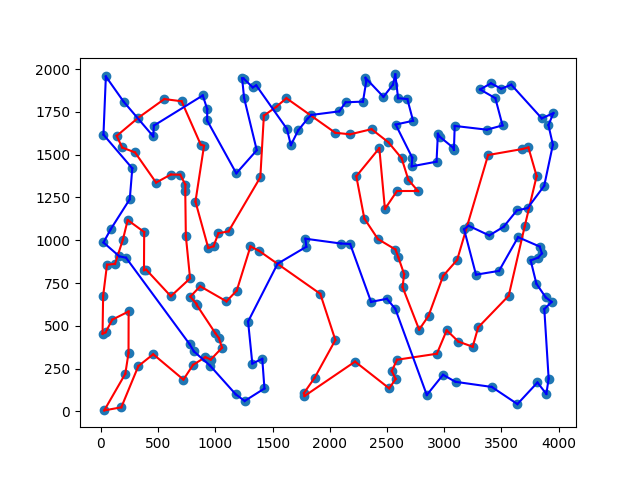
\includegraphics[width=\linewidth]{best_paths/kroA200/traverse_steepest_edge}
        \caption{kroA200, losowy start}
    \end{minipage}
    \hfill
    \begin{minipage}[t]{0.45\textwidth}
        \centering
        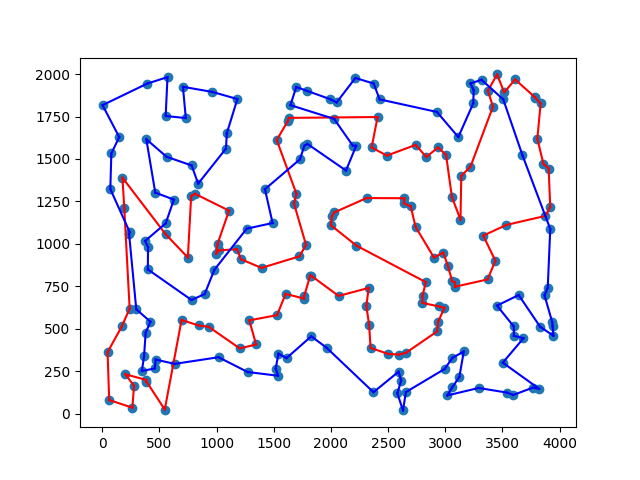
\includegraphics[width=\linewidth]{best_paths/kroB200/traverse_steepest_edge}
        \caption{kroB200, losowy start}
    \end{minipage}\label{fig:figure1}
\end{figure}


\subsubsection{Algorytm stromy z listą ruchów}\label{subsubsec:algorytm-stromy-z-lista-ruchow}

\begin{figure}[H]
    \begin{minipage}[t]{0.45\textwidth}
        \centering
        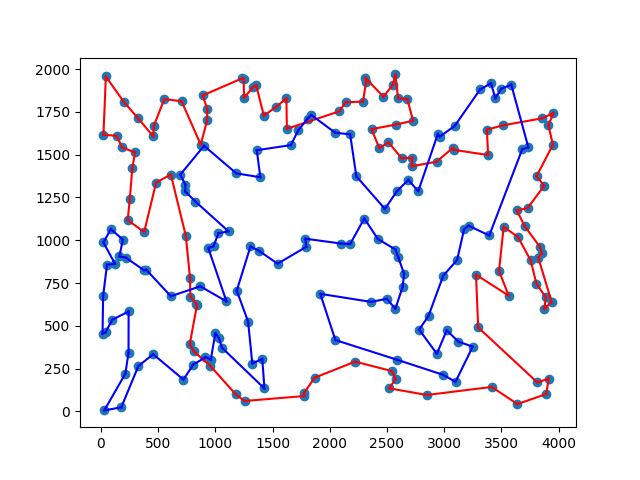
\includegraphics[width=\linewidth]{best_paths/kroA200/steepest_LM}
        \caption{kroA200, losowy start}
    \end{minipage}
    \hfill
    \begin{minipage}[t]{0.45\textwidth}
        \centering
        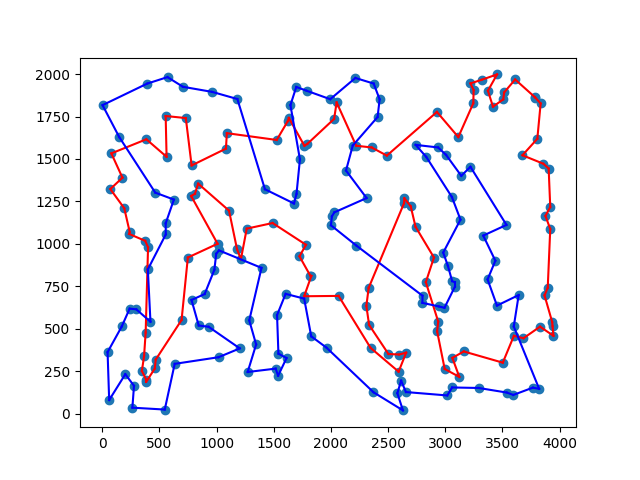
\includegraphics[width=\linewidth]{best_paths/kroB200/steepest_LM}
        \caption{kroB200, losowy start}
    \end{minipage}\label{fig:figure2}
\end{figure}


\subsubsection{Algorytm stromy z mechanizmem ruchów kandydackich}\label{subsubsec:algorytm-stromy-z-mechanizmem-ruchow-kandydackich}

\begin{figure}[H]
    \begin{minipage}[t]{0.45\textwidth}
        \centering
        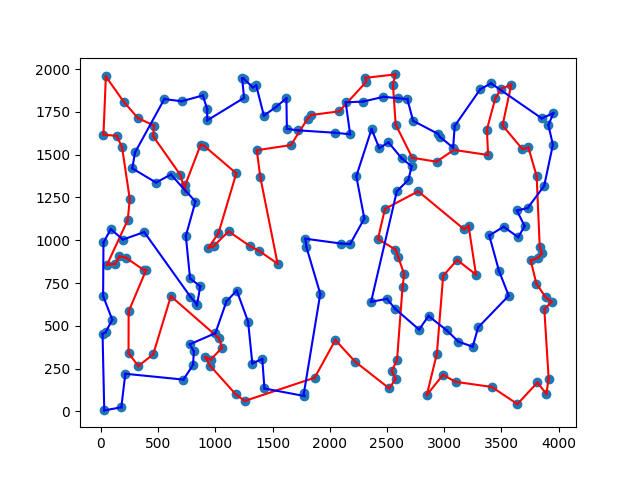
\includegraphics[width=\linewidth]{best_paths/kroA200/steepest_kandydackie}
        \caption{kroA200, losowy start}
    \end{minipage}
    \hfill
    \begin{minipage}[t]{0.45\textwidth}
        \centering
        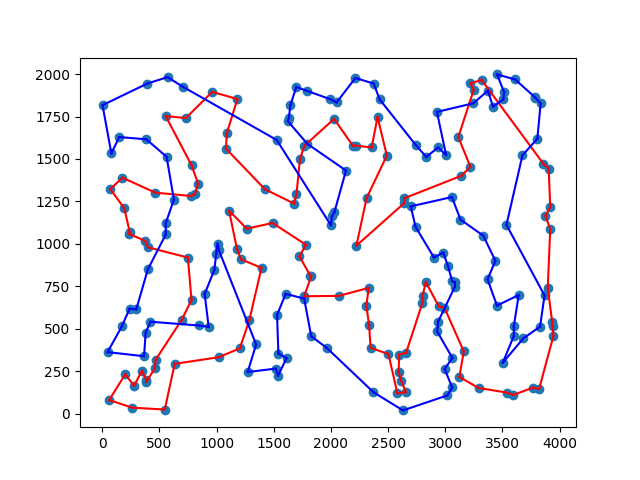
\includegraphics[width=\linewidth]{best_paths/kroB200/steepest_kandydackie}
        \caption{kroB200, losowy start}
    \end{minipage}\label{fig:figure3}
\end{figure}


\subsubsection{Heurystyka konstrukcyjna}\label{subsubsec:heurystyka-konstrukcyjna}

\begin{figure}[H]
    \begin{minipage}[t]{0.45\textwidth}
        \centering
        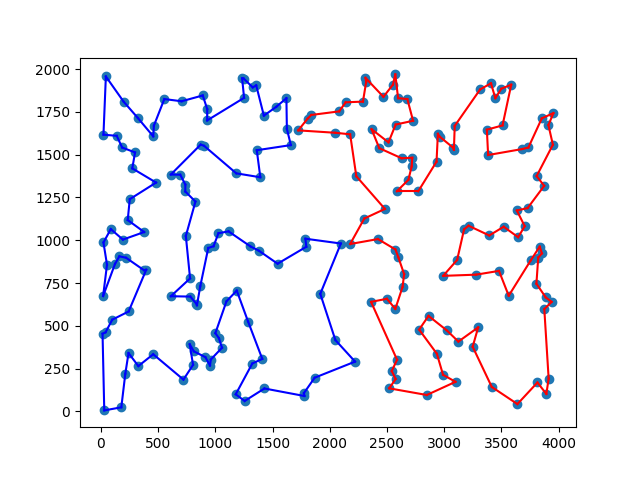
\includegraphics[width=\linewidth]{best_paths/kroA200/split_paths_regret_TSP}
        \caption{kroA200, losowy start}
    \end{minipage}
    \hfill
    \begin{minipage}[t]{0.45\textwidth}
        \centering
        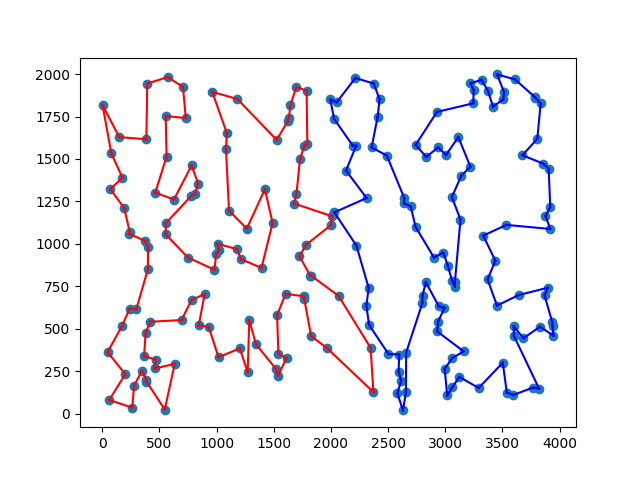
\includegraphics[width=\linewidth]{best_paths/kroB200/split_paths_regret_TSP}
        \caption{kroB200, losowy start}
    \end{minipage}\label{fig:figure4}
\end{figure}


\section{Wnioski i analiza wyników}\label{sec:wnioski}

Na podstawie wyników można zauważyć, że algorytm stromy z listą ruchów oraz algorytm stromy z mechanizmem ruchów kandydackich są znacznie bardziej efektywne niż algorytm bazowy.
W przypadku instancji kroA200 algorytm stromy z listą ruchów osiągnął lepszy wynik, natomiast w przypadku instancji kroB200 algorytm stromy z mechanizmem ruchów kandydackich okazał się lepszy.
Niezależnie od instancji algorytm korzystający z ruchów kandydackich okazał się odrobinę bardziej efektywny czasowo.
Wyniki naszej heurystyki konstrukcyjnej są wciąż najlepsze, jednak jest to przede wszystkim zasługa dobrego startowego podziału, czyli zastosowania swego rodzaju wiedzy dziedzinowej,
a to sugeruje, że algorytmy lokalnego przeszukiwania mogą być użyte do poprawy wyników heurystyki konstrukcyjnej, ale nie jako osobna metoda znajdowania optimum rozpoczynając z rozwiązań losowych.
Poprzednie zadanie pokazało, że algorytmy lokalnego przeszukiwania są bardziej efektywne w przypadku, gdy startujemy z rozwiązań konstrukcyjnych.


\section{Link do repozytorium}\label{sec:link-do-repo}
Kod źródłowy w repozytorium GitHub dostępny pod linkiem: \\
\href{https://github.com/KotZPolibudy/PUT_IMO/tree/main/Lab3%20-%20Local_augmented}{Repozytorium}.

\end{document}
